%!TEX root = ./main.tex

\section[In the Field]{Surfaces, Trains, and Lasers}

% SECTION TIMING: 52:00--64:00 (7 frames).
% The DISCO frames are the security payoff of the lecture. If time is short, cut the
% two FSO frames instead -- the attack is the part students remember.

\begin{frame}{A surface that edits the channel}
  \vspace{0.4em}
  \centering
  \begin{tikzpicture}[scale=0.92,transform shape]
    \node[netnode,minimum width=1.6cm] (bs) at (0,0) {BS};
    \node[netnode,minimum width=1.6cm] (ue) at (6.0,0) {User};
    \node[oranode,minimum width=2.0cm] (ris) at (3.0,1.9) {RIS};
    \draw[flow,draw=softgray,dashed] (bs) -- node[font=\scriptsize,below]{blocked / weak} (ue);
    \draw[flow,draw=ranpurple,very thick] (bs) -- (ris);
    \draw[flow,draw=ranpurple,very thick] (ris) -- (ue);
    \node[font=\scriptsize,text=ranpurple,anchor=east] at (1.25,1.45) {passive};
    \node[font=\scriptsize,text=ranpurple,anchor=west] at (4.75,1.45) {no amplifier};
  \end{tikzpicture}

  \vspace{0.9em}
  \begin{columns}[T,onlytextwidth]
    \column{0.47\textwidth}
      {\small\textbf{\textcolor{softgreen}{Used honestly}} it adds coverage, energy
       efficiency, and a second look at a target.\par}
    \column{0.47\textwidth}
      {\small\textbf{\textcolor{ranpurple}{Used dishonestly}} it changes your channel
       without ever emitting a signal of its own.\par}
  \end{columns}

  \glossline{RIS = Reconfigurable Intelligent Surface \quad
    SE / EE = Spectral / Energy Efficiency}
\end{frame}

% ACCURACY NOTE: a DISCO RIS is a FULLY PASSIVE jammer. It has no transmitter and no
% knowledge of the legitimate channels. It jams by re-randomising its phase shifts fast
% enough that the CSI the BS estimated is already stale -- "active channel aging".
% Do not describe it as "transmitting noise". That is the entire novelty.
\begin{frame}{The jammer that never transmits}
  \vspace{0.3em}
  \centering
  \begin{tikzpicture}[scale=0.90,transform shape]
    \node[netnode,minimum width=1.7cm] (bs) at (0,0) {ISAC BS};
    \node[netnode,minimum width=1.5cm] (ue) at (6.2,0.9) {User};
    \node[corenode,minimum width=1.5cm] (tg) at (6.2,-0.9) {Target};
    \node[oranode,minimum width=2.4cm] (dris) at (3.1,2.0) {DISCO RIS\\[-2pt]{\scriptsize no transmitter}};
    \draw[flow,draw=ranblue] (bs) -- (ue);
    \draw[flow,draw=coreorange] (bs) -- (tg);
    \draw[flow,draw=ranpurple,very thick] (bs) -- (dris);
    \draw[flow,draw=ranpurple,very thick] (dris) -- (ue);
    \draw[flow,draw=ranpurple,very thick] (dris) to[bend left=12] (tg);
    \node[font=\scriptsize,text=ranpurple,anchor=south] at (3.1,2.55)
      {phases re-randomised every frame};
  \end{tikzpicture}

  \vspace{0.7em}
  \qa{How do you jam a link with no amplifier and no channel knowledge?}
     {By making the channel move. The base station beamforms on estimated CSI; a
      surface that reshuffles itself faster than the estimate refreshes turns that
      CSI stale on arrival. The published name for it is \textbf{active channel aging}.}

  \source{https://ieeexplore.ieee.org/document/10681452}{H. Huang et al., ISAC under DISCO physical-layer jamming attacks, IEEE WCL 13(11), 2024}
\end{frame}

\begin{frame}{What the attack actually breaks}
  \vspace{0.5em}
  \begin{columns}[T,onlytextwidth]
    \column{0.30\textwidth}
      {\small\textbf{\textcolor{softgray}{Without the attack}}\par}
      \vspace{0.4em}
      {\small A well-designed ISAC waveform costs the sum-rate very little. Sensing is
       nearly free.\par}
    \column{0.34\textwidth}
      {\small\textbf{\textcolor{ranpurple}{With a DISCO RIS}}\par}
      \vspace{0.4em}
      {\small Both functions degrade at once, and the victim has no knowledge of the
       jammed channel to correct with.\par}
    \column{0.30\textwidth}
      {\small\textbf{\textcolor{softgreen}{What helps}}\par}
      \vspace{0.4em}
      {\small The damage is statistical, so it can be quantified --- and what can be
       quantified can be budgeted for.\par}
  \end{columns}

  \vspace{0.8em}
  \glossline{ACA = Active Channel Aging \quad CSI = Channel State Information \quad
    MUI = Multi-User Interference}

  \vspace{0.2em}
  \takeaway{A passive attacker leaves no emission to detect.\\Your only evidence is your own falling SINR.}
\end{frame}

% SOURCE: Panpan Li, Yong Niu, Hao Wu, Zhu Han, Ning Wang, Lei Xiong, Bo Ai, Chau Yuen,
% "Secure High-Speed Train-to-Ground Communications Through ISAC," IEEE Internet of
% Things Journal, vol. 11, no. 19, pp. 31235-31248, October 2024.
\begin{frame}{350 km/h is a hostile radio environment}
  \begin{columns}[T,onlytextwidth]
    \column{0.42\textwidth}
      \centering
      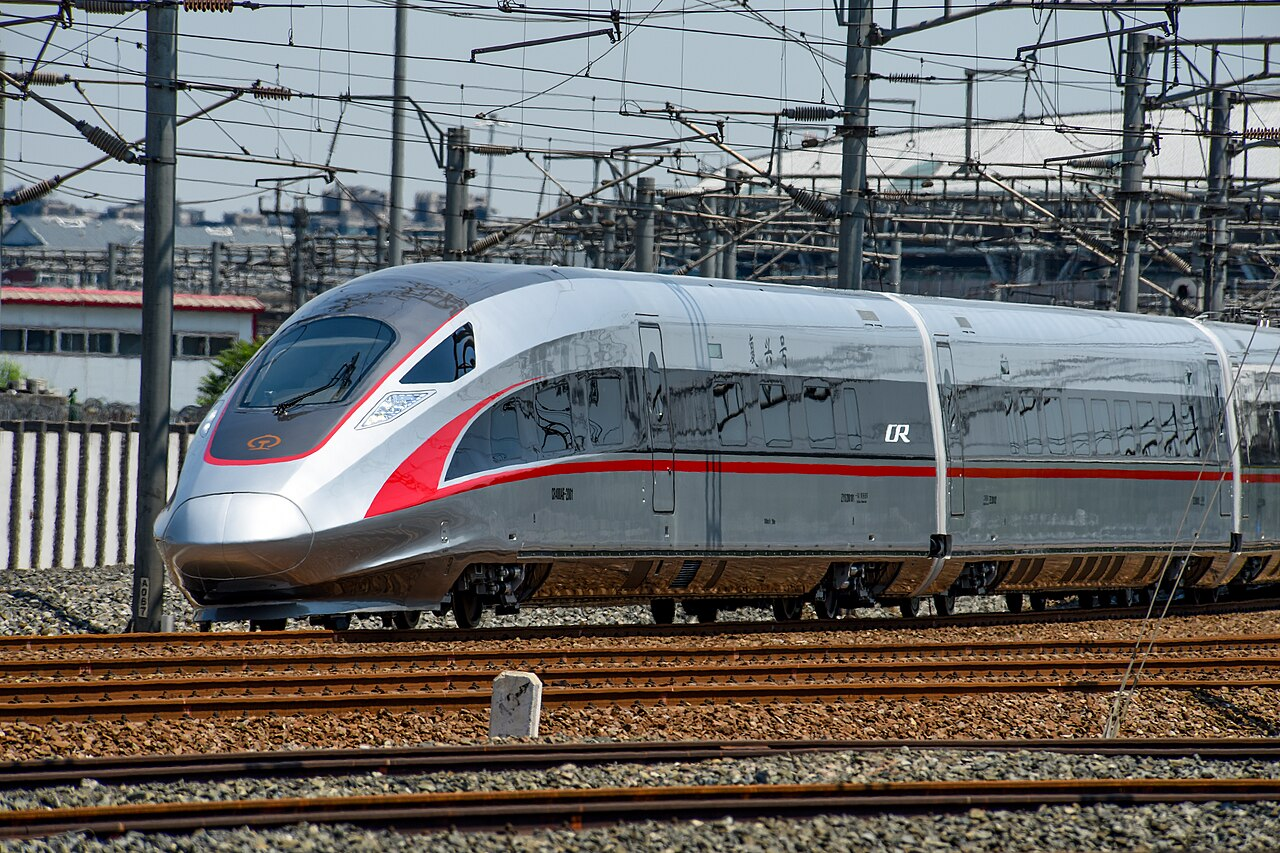
\includegraphics[width=\linewidth]{figure/isac/hsr_cr400af.jpg}
      \source{https://commons.wikimedia.org/wiki/File:CR400AF-2001@BJN_(20170626110730).jpg}{CR400AF high-speed trainset}
    \column{0.54\textwidth}
      \small
      \begin{itemize}\itemsep5pt
        \item mmWave blocks on anything.
        \item Doppler is large and shifting.
        \item Handovers every few seconds.
        \item The track must be watched too.
      \end{itemize}

      \vspace{0.5em}
      {\small\textcolor{coreorange}{\textbf{One system carries passengers and
       watches the line.}}\par}
  \end{columns}

  \vspace{0.3em}
  \takeaway{Rooftop relays turn one hard outdoor link\\into one easy link plus an indoor problem.}
\end{frame}

% ACCURACY NOTE: the "blind region" is a secrecy constraint -- the beam design
% deliberately keeps an eavesdropper region poorly illuminated. It is not a coverage hole
% caused by blockage. Students conflate the two.
\begin{frame}{Beamforming with a deliberate blind spot}
  \vspace{0.3em}
  \centering
  \begin{tikzpicture}[scale=0.88,transform shape]
    \node[netnode,minimum width=1.9cm] (bs) at (0,0) {ISAC BS};
    \node[netnode,minimum width=1.9cm] (mr) at (4.8,1.35) {Mobile relay};
    \node[oranode,minimum width=1.9cm] (ev) at (4.8,-1.35) {Eavesdropper};
    \draw[flow,draw=ranblue,very thick] (bs)
      -- node[font=\scriptsize,text=ranblue,sloped,above,pos=0.55]{main lobe} (mr);
    \draw[flow,draw=softgray,dashed] (bs)
      -- node[font=\scriptsize,text=softgray,sloped,below,pos=0.34]{blind region, by design} (ev);
    \node[align=center,font=\scriptsize,anchor=south] at (4.8,2.05) {carriage roof to cabin Wi-Fi};
  \end{tikzpicture}

  \vspace{0.7em}
  \begin{columns}[T,onlytextwidth]
    \column{0.47\textwidth}
      {\small\textbf{Two variables}\par}
      \vspace{0.3em}
      {\small Beamforming matrix, for where the energy points. Waveform, for what the
       energy says.\par}
    \column{0.47\textwidth}
      {\small\textbf{Four constraints}\par}
      \vspace{0.3em}
      {\small Transmit power, constant modulus, sensing SINR, and the blind
       region.\par}
  \end{columns}

  \source{https://ieeexplore.ieee.org/document/10557622}{P. Li et al., Secure High-Speed Train-to-Ground Communications Through ISAC, IEEE IoT J. 11(19), 2024}
\end{frame}

% SOURCE: FSO-ISAC section. Research gap as stated in the source talk: existing FSO-ISAC
% work is mostly pulsed or single-carrier; multicarrier is underexplored.
\begin{frame}{The same argument, in light}
  \begin{columns}[T,onlytextwidth]
    \column{0.40\textwidth}
      \centering
      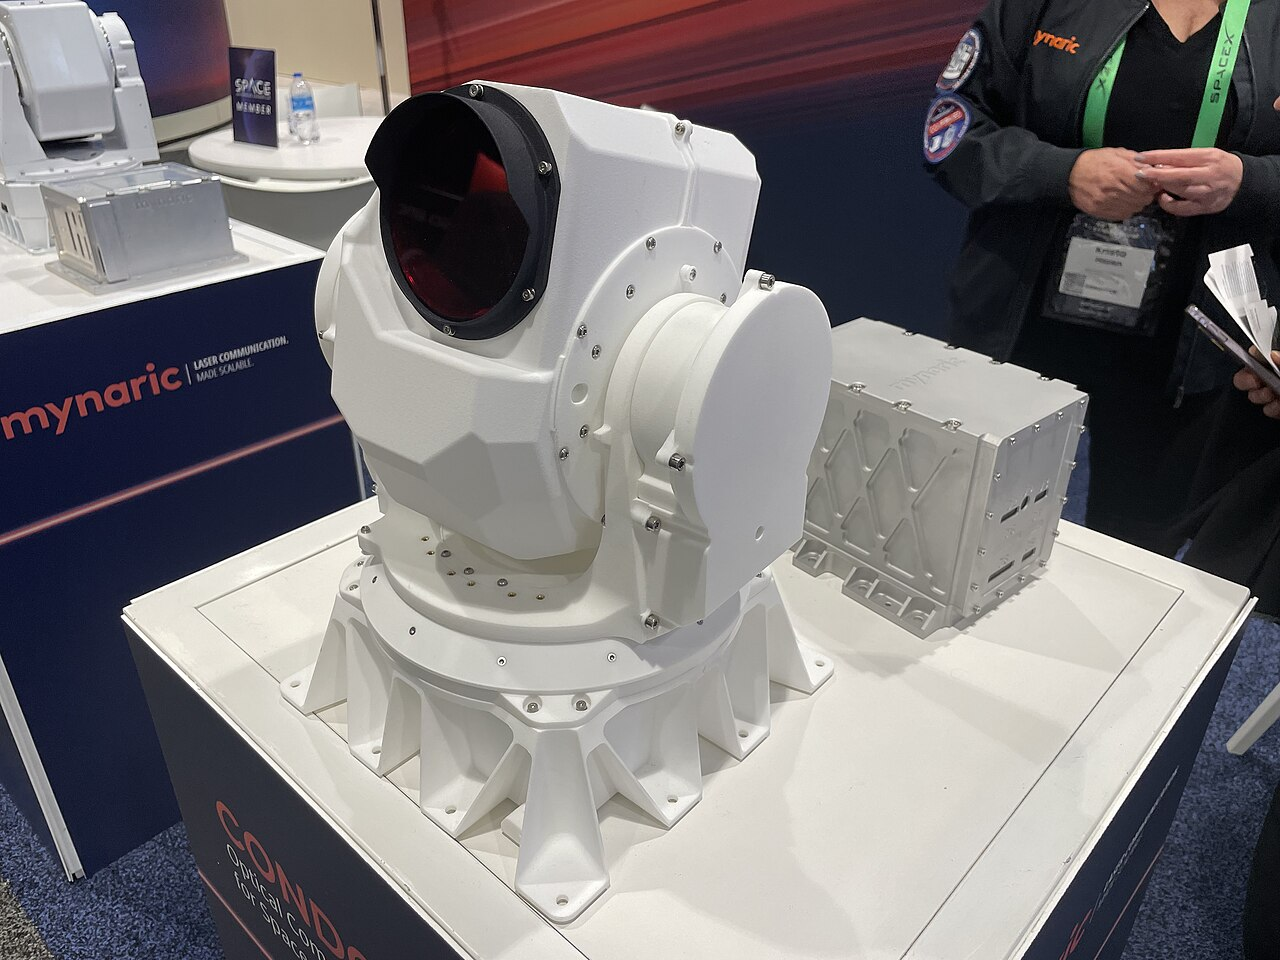
\includegraphics[width=\linewidth]{figure/isac/fso_terminal.jpg}
      \source{https://commons.wikimedia.org/wiki/File:Mynaric_Condor_Mk3.1_Satellite_optical_communication_terminal.jpg}{Optical communication terminal, 2025}
    \column{0.56\textwidth}
      \small
      \begin{itemize}\itemsep4pt
        \item LiDAR already ranges with light.
        \item An optical link already carries data.
        \item Same aperture, detector, and beam.
        \item No RF licence to argue about.
      \end{itemize}

      \vspace{0.6em}
      \qa{Why does an optical system need a DC bias?}
         {Because intensity cannot be negative. The bias lifts the waveform above
          zero --- and every watt of bias carries no information.}
  \end{columns}

  \glossline{FSO = Free Space Optics \quad LiDAR = Light Detection and Ranging\\
    IM/DD = Intensity Modulation / Direct Detection \quad
    DCO-OFDM = DC-biased Optical OFDM}
\end{frame}

% ACCURACY NOTE: the interesting finding is the SHAPE of the curve, not the numbers.
% Both metrics saturate, so near either end you pay a lot for very little.
\begin{frame}{The same curve, drawn in photons}
  \vspace{0.3em}
  \begin{columns}[T,onlytextwidth]
    \column{0.46\textwidth}
      \centering
      \begin{tikzpicture}[scale=0.88,transform shape]
        \draw[-{Latex[length=2.2mm]},softgray] (0,0) -- (3.9,0);
        \node[font=\scriptsize,anchor=north] at (2.0,-0.08) {ranging precision $\rightarrow$};
        \draw[-{Latex[length=2.2mm]},softgray] (0,0) -- (0,2.9);
        \node[font=\scriptsize,rotate=90,anchor=south] at (-0.18,1.45) {spectral efficiency};
        \draw[very thick,draw=ranblue] (0.35,2.55) .. controls (1.6,2.45) and (2.2,1.8) .. (3.3,0.4);
        \node[font=\scriptsize,text=softgray,anchor=south west] at (0.45,2.62) {flat: cheap};
        \node[font=\scriptsize,text=coreorange,anchor=west] at (3.0,1.05) {cliff};
      \end{tikzpicture}
    \column{0.50\textwidth}
      \small
      \begin{itemize}\itemsep5pt
        \item Tune DC bias with the powers.
        \item Rate is the objective.
        \item Precision is the constraint.
        \item Both metrics saturate.
      \end{itemize}
  \end{columns}

  \vspace{0.6em}
  \takeaway{The right question is never ``which is better''.\\It is ``where on the curve is the cliff''.}
\end{frame}
